%!TEX root=../../template.tex
\section{Optical Systems}%
\label{sec:theobg_opticalsystems}

Optical systems are, as far as this thesis is concerned, light capturing
and digitising systems. Their purpose is to gather light from the
environment at certain conditions and format it into data that one can
analyse computationally and a general schematic representation is
presented in Figure~\ref{fig:theobg_opticalsystems_generalschematic}.
In this section, I will present the basic theoretical concepts on which
I stood to design the optical system, as it is presented in the
following chapters. 

\begin{figure}[htpb]
    \centering
    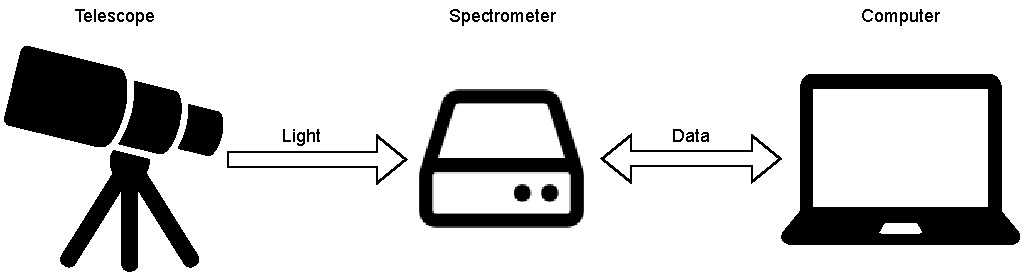
\includegraphics[width=.8\textwidth]{img/pdf/opticalSystemBasic.drawio.pdf}
    \caption{General schematic for an optical system, as relevant to the
    work of this thesis. Its function is to gather environment light and
    format it as data.}%
    \label{fig:theobg_opticalsystems_generalschematic}
\end{figure}

\subsection{Telescopes}%
\label{sub:theobg_opticalsystems_telescopes}

The most basic form of telescope comes from the juxtaposition of two
lenses~\cite{Hecht2016}, as depicted in
Figure~\ref{fig:basic_telescope}. The focal point of the objective is
coincident with the focal point of the eyepiece. Notice, also from the
figure, that the rays reaching in the eye are parallel, so the observer
can use the telescope with a relaxed eye~\cite{Hecht2016}.

\begin{figure}[htpb]
    \centering
    % \includegraphics[width=0.8\linewidth]{name.ext}
    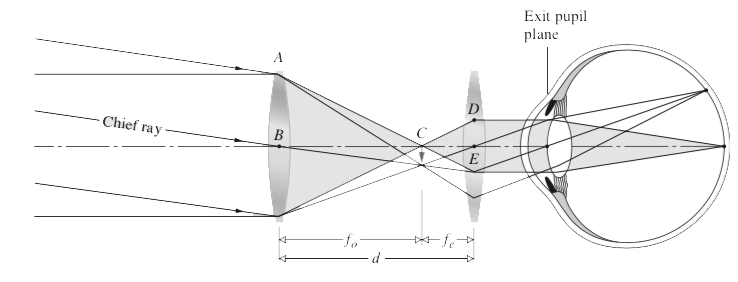
\includegraphics[width=0.8\linewidth]{img/png/telescope.png}
    \caption{The most basic form of telescope. The second lens
    (eyepiece) magnifies the image produced by the first lens (the
    objective)~\cite{Hecht2016}}%
    \label{fig:basic_telescope}
\end{figure}

It is a simple conceptual operating principle. The idea is to have a
device that directionally captures ambient light and direct it into an
observer's eye (or optical sensor). The amount of captured light that is
captured depends on the section of the first lens, the objective (think of a constant
stream of photons entering a bucket-like device). Telescopes come in
various sizes and shapes. As so many devices, telescopes vary with the
application the designer had in mind. Astronomical telescopes produce
inverted images. This would be highly confusing for terrestrial
observations (therefore, terrestrial telescopes have an erector lens).
There are two main types of telescope, refractors (see
Figure~\ref{fig:basic_telescope}) and reflectors (see
Figure~\ref{fig:reflector_telescopes}). While conceptually much simpler,
refraction based telescopes do have several drawbacks. They are
exclusively dependent on lenses, which are difficult to manufacture.
Their magnification also only depends on the length of the telescope's
tube, which makes them unwieldy very quickly as large magnification
implies long tubes. These inconveniences are in part solved by
reflecting telescopes. They are less vulnerable to fabrication defects,
since mirrors are much easier to produce than lenses. This brings the
added benefit of having wider objectives and thus much more light
entering the tube. Of at least the same importance, the focal length's
dependence of the length of the tube dissipates, since the light path
between the objective and the observer's eye depends now on the mirror
configuration inside the telescope. For all these advantages, there are
nowadays no great telescopes of refracting geometry~\cite{Smith2000,
Hecht2016}.

\begin{figure}[htpb]
    \centering
    % left bottom right top
    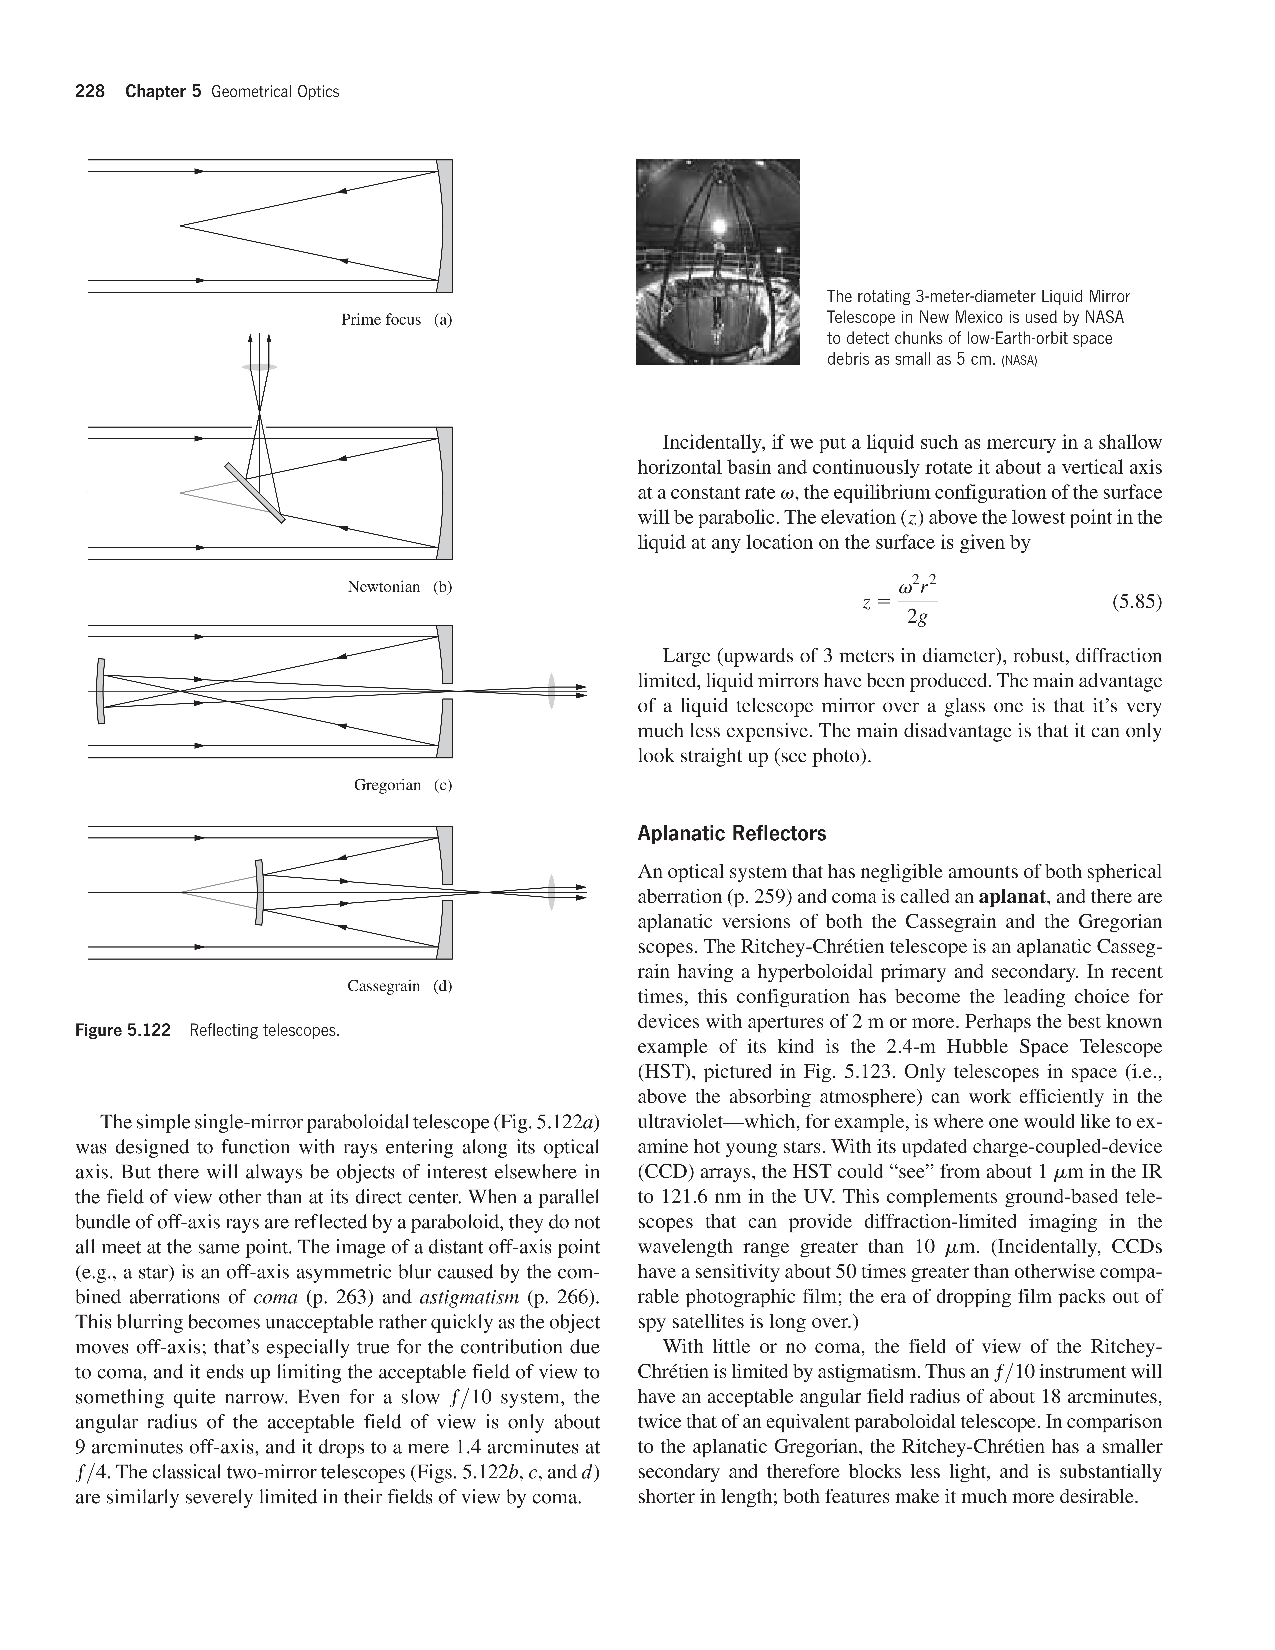
\includegraphics[clip,%
    trim=1cm 11.5cm 11cm 13.5cm,%
    width=.8\textwidth]{img/pdf/optics_reflector_telescopes_235.pdf}
    \caption{A refractor telescope of the Cassegrain
    variant~\cite{Hecht2016}.}\label{fig:reflector_telescopes}
\end{figure}


\subsection{Spectrometers}%
\label{sub:theobg_opticalsystems_spectrometers}

Spectrometers are devices that measure and relate the intensity and
colour of a given radiation source. In other words, it is sensitive to
both the quantity and the energy of this radiation source's photons.
There are many types of spectrometers. They differ on the energy range
of the radiation they can measure, on the physical principle they are
based on, on their applications and on the geometry of their internal
components. In this thesis, the only type of spectrometer that was used
a UV-Vis Czerny-Turner spectrometer. A schematic representation of this
type of spectrometer is presented in
Figure~\ref{fig:czernyturner}~\cite{Neumann2014}, and a more realistic
representation is displayed in
Figure~\ref{fig:avantes_3d}~\cite{Avantes2022}. As can be seen in both
schematics, light enters the assembly through the slit and is collimated
on a spherical mirror, which reflects it towards an oriented diffraction
grating. The resulting diffracted light is then focused on a second
spherical mirror onto a 1D linear detector array.  This particularly
optical assembly is highly customisable. One can choose between a
variety of sensors, diffraction gratings and entrance slits, according
to the spectral parameters required for one's experiment or application.
Here are the most important of them.

\begin{description}
    \item[Optical Resolution] The optimal resolution comes from a
        correct balance between slit size and diffraction grating.
        Normally, for a high resolution application one would opt by
        using a high number of lines for the diffraction grating and a
        very small slit. Choose an excessive number of lines and the
        wavelength becomes too limited; choose an excessively small slit
        and there will not be enough light going through the system;
    \item[Sensitivity] photometric sensitivity (how much light do we
        need to get a signal) and chemometric sensitivity (the smallest
        absorbance difference that can be measured by the device) are
        important device features that need to be considered
        \emph{a-priori};
    \item[Sensor / Detector] the type of measurement being made
        determines the types of sensors that can be used. For instance,
        faster detectors are normally good choices in abundant light
        conditions that allow for lower integration times.
\end{description}

\begin{figure}
    \centering
      \begin{subfigure}[a]{.8\linewidth}
        \centering
        % left bottom right top
        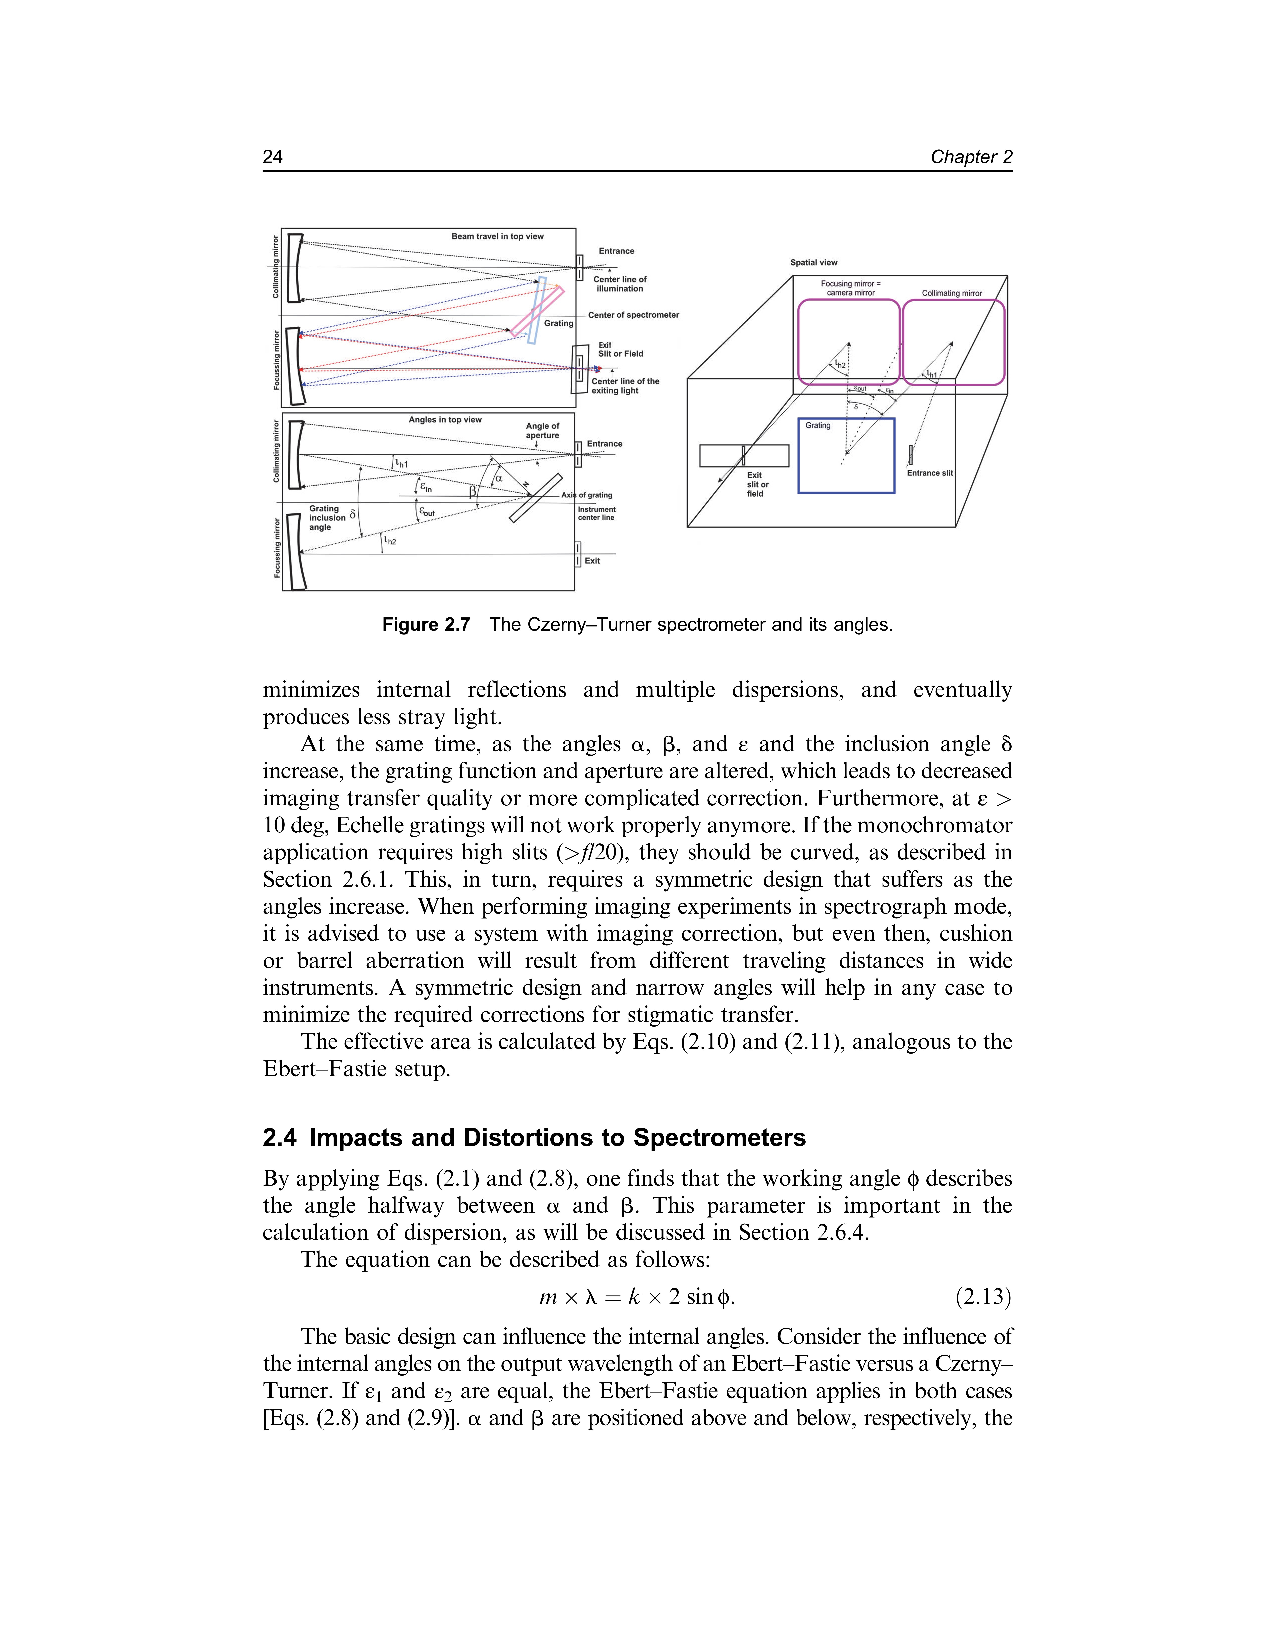
\includegraphics[clip,%
        trim=3.7cm 17.5cm 3.7cm 3.7cm,%
        width=.8\textwidth]{img/pdf/neumannCzernyTurner.pdf}
        \caption{The definition schematic for the Czerny-Turner
        spectrometer, including all the relevant
        angles~\cite{Neumann2014}}\label{fig:czernyturner}
      \end{subfigure}%
      \\
      \begin{subfigure}[b]{.6\linewidth}
        \centering
        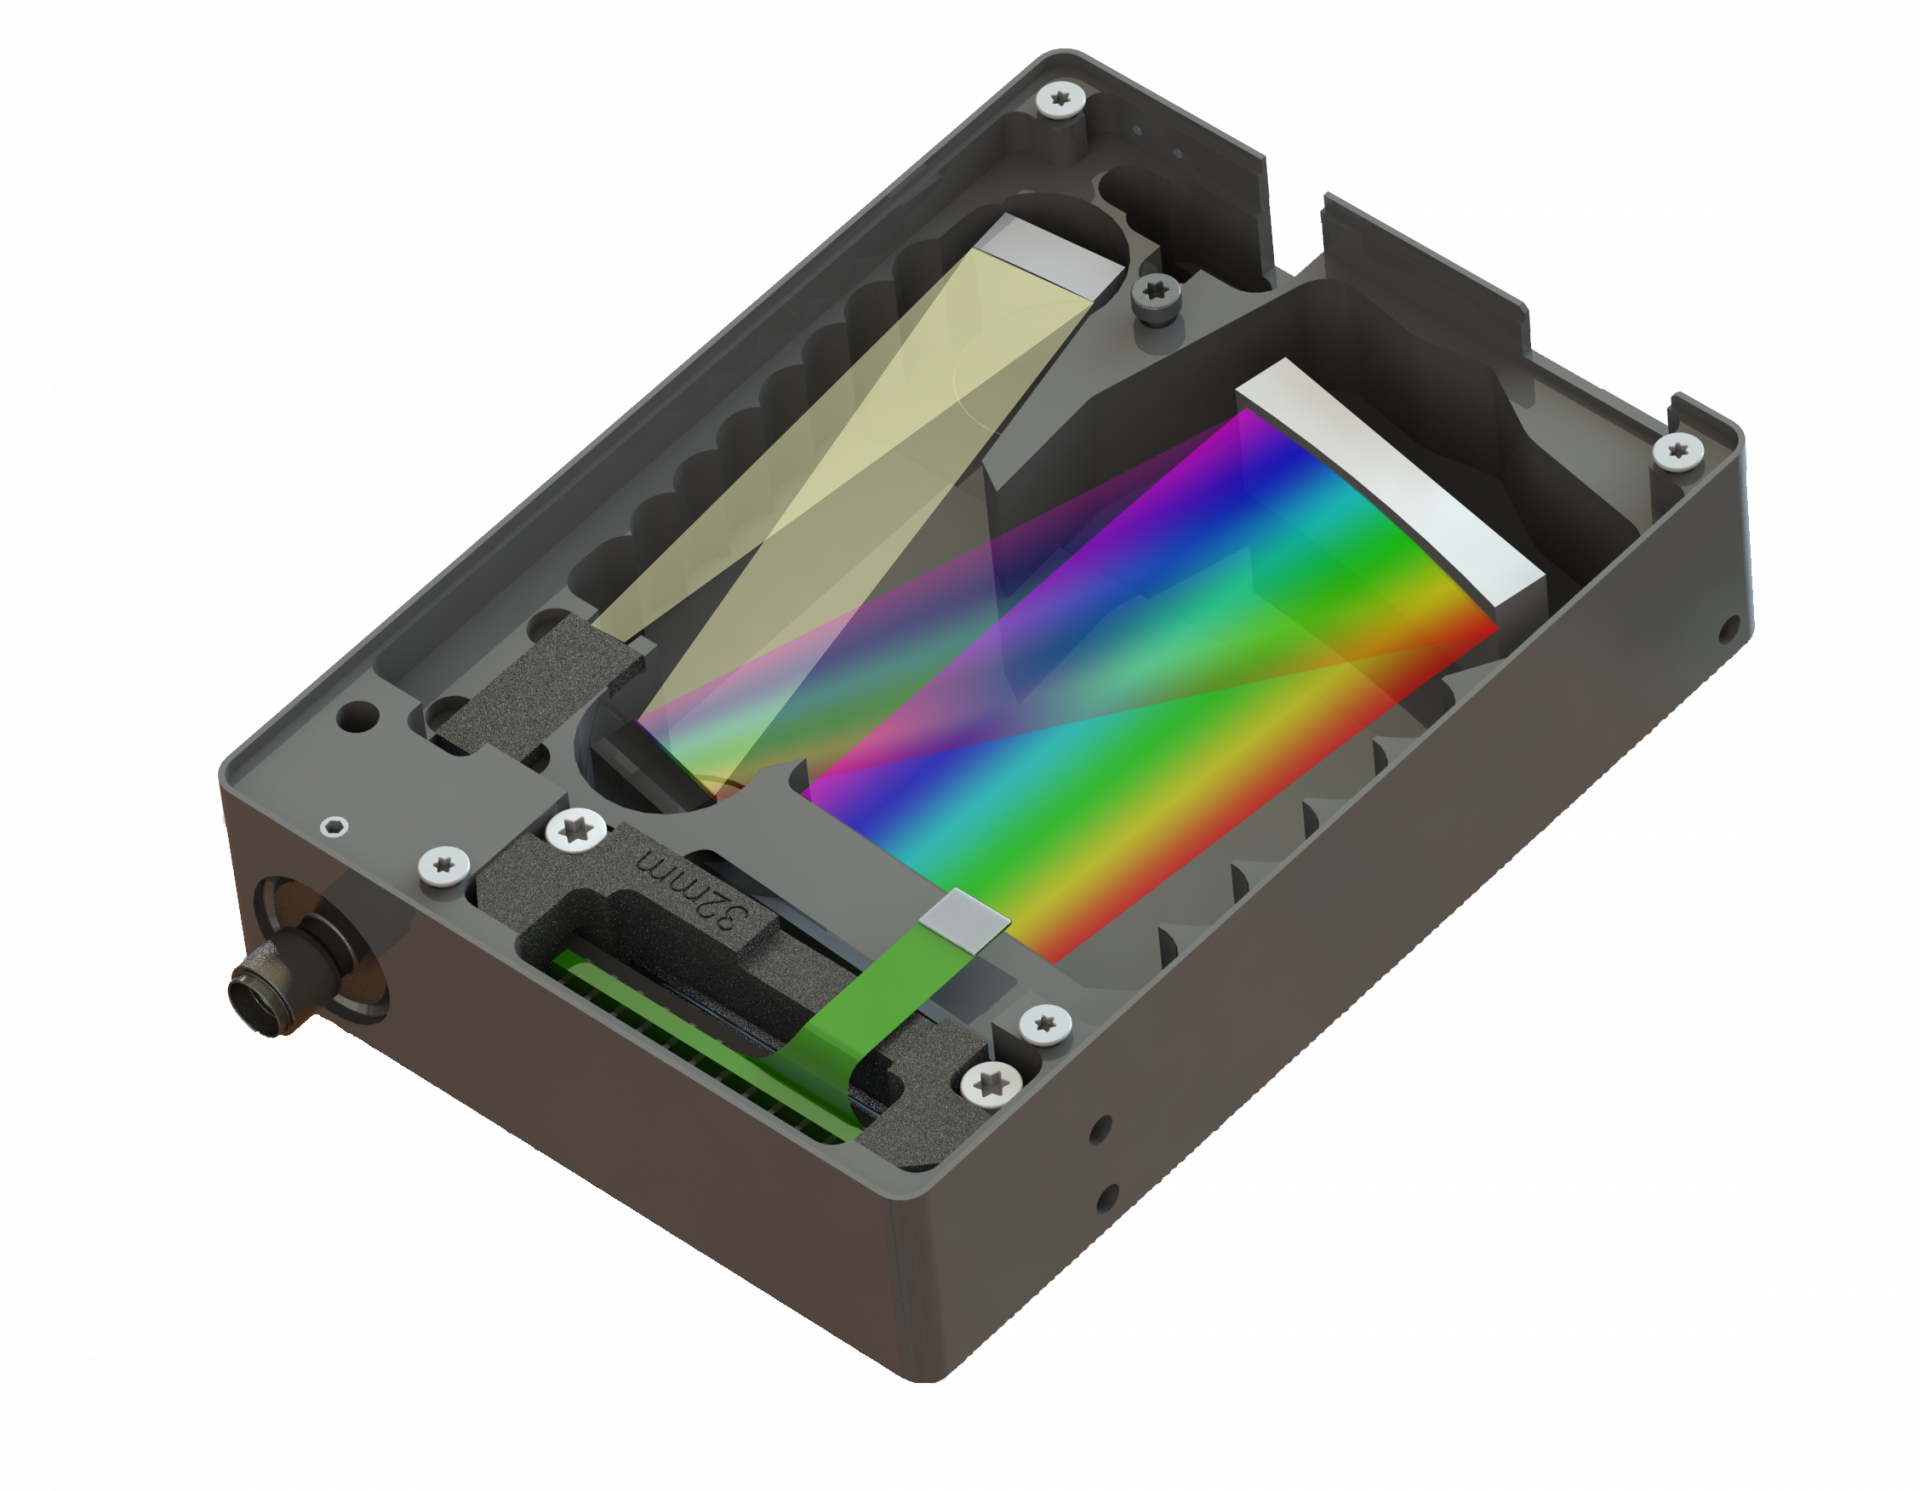
\includegraphics[width=.8\textwidth]{img/png/Open-Bench-V2.png}
        \caption{The optical bench of an Avantes
        spectrometer~\cite{Avantes2022}.}\label{fig:avantes_3d}
      \end{subfigure}
      \caption{Basic schematics for the two types of telescopes
      presented.}\label{fig:telescope_types_schematics}
\end{figure}

Finally, the choice of spectrometer should also include into
consideration some less desirable, but inescapable,  features of these
devices. The most important of these is the thermal stability.
Temperature variation produces slight changes in the spectrometer's
optical bench and surrounding structures, which means that each part of
the detector is exposed to a slightly different section of the spectrum,
which naturally leads to different signal results. Commercial
spectrometer manufacturers normally provide quality control measurements
for the device's thermal stability
values~\cite{Merlaud2013, Avantes2022}.
